%----------------------------------------------------------------------------------------
%	PACKAGES AND DOCUMENT CONFIGURATIONS
%----------------------------------------------------------------------------------------

\documentclass[12pt,letter]{article}
\usepackage[utf8]{inputenc}


% Adjusting margins to personal my need
\addtolength{\oddsidemargin}{-.5in}
\addtolength{\evensidemargin}{-.5in}
\addtolength{\textwidth}{1in}
\addtolength{\topmargin}{-.5in}
\addtolength{\textheight}{1in}

% Graphics
\usepackage{caption}
\usepackage{subcaption}
\usepackage{graphicx}
\graphicspath{{figures/}}

% Math
\usepackage{amssymb}
\usepackage{amsmath} % Required for some math elements 

% Other
\usepackage{algorithm}
\usepackage{algorithmic}
\usepackage{array}
\usepackage{lipsum}
\usepackage{hyperref}

\hypersetup{
    colorlinks=true,
    linkcolor=blue,
    filecolor=magenta,
    urlcolor=blue,
}
\usepackage{forest}
\forestset{
    default preamble={
        for tree={circle,draw}
    }
}


%----------------------------------------------------------------------------------------
%	MAIN PART
%----------------------------------------------------------------------------------------
\begin{document}

    \title{Stroke Predictions} % Title
    \author{Chathumini Abeyratna, Saadiya Allahbaksh, Kevin Karnani}
    \date{\today} % Date for the report
    \maketitle % Inserts the title, author and date


%----------------------------------------------------------------------------------------
%	Abstract
%----------------------------------------------------------------------------------------
    \begin{abstract}
        \normalsize
%% Text of the abstract
        We were curious to see the effect that certain features had in the possibility of a person having a stroke and how well machine learning models predicted stroke. We decided to dive deep into the background research we found, any related work we came across, the dataset we will be using, and the machine learning models that we created to predict stroke based on features. We found that for many cases, \verb|Age| contributed the most to strokes, followed by \verb|BMI| and \verb|Smoking_Status|. Conversely, factors like \verb|Ever_Married|, \verb|Gender|, \verb|Hypertension|, and \verb|Heart_Disease| had little to no effect on strokes.

    \end{abstract}

%----------------------------------------------------------------------------------------
%	Table of Content
%----------------------------------------------------------------------------------------
    \setcounter{tocdepth}{5}
    \setcounter{secnumdepth}{5}
    \newpage
    \tableofcontents


    \clearpage

%----------------------------------------------------------------------------------------
%	Main Part
%----------------------------------------------------------------------------------------
    \section{Introduction}
\label{sec:introduction}

The World Health Organization (WHO) identifies strokes as the second leading cause of death globally \cite{WHO}. A stroke happens when a person's blood supply to their brain is interrupted or reduced, causing brain cells to die within minutes. It prevents the brain tissue from getting the oxygen and nutrients that it needs and is responsible for approximately 11\% of total deaths. To see what effect certain factors had on people who suffered strokes, we decided to create 3 Machine Learning Models: Logistic Regression, Support Vector Machines, and Random Forest. We did this by not only writing our own code to create the models, but we also compared the yielded metrics to those from built-in models of \verb|Scikit-Learn|, a built-in Machine Learning Python library.

    \section{Dataset}
\label{sec:dataset}
The dataset that we will be using for the models were taken from Kaggle \cite{Kaggle}. There are 5110 entries of individuals, their relevant feature details, and whether they had a stroke or not.

\subsection{Columns}
\label{sec:dataset:Columns}
\begin{itemize}
    \item \verb|id|: unique identifier
    \item \verb|gender|: "Male", "Female" or "Other"
    \item \verb|age|: age of the patient
    \item \verb|hypertension|: 0 if the patient doesn't have hypertension, 1 if the patient has hypertension
    \item \verb|heart_disease|: 0 if the patient doesn't have any heart diseases, 1 if the patient has a heart disease
    \item \verb|ever_married|: "No" or "Yes"
    \item \verb|work_type|: "children", "Govt\_jov", "Never\_worked", "Private" or "Self-employed"
    \item \verb|Residence_type|: "Rural" or "Urban"
    \item \verb|avg_glucose_level|: average glucose level in blood
    \item \verb|bmi|: body mass index
    \item \verb|smoking_status|: "formerly smoked", "never smoked", "smokes" or "Unknown"
    \item \verb|stroke|: 1 if the patient had a stroke or 0 if not

\end{itemize}

    \section{Methodology}
\label{sec:methodology}

Since we have three members, we decided to tackle the project by assigning a machine learning model to each member. Chathumini focused on creating the Logistic Regression model, while also exploring the differences between batch and stochastic gradient descent and implementing k-fold cross validation. Saadiya worked on creating the SVM model and plotting their Precision-Recall Curves. Kevin implemented the ID3 and Random Forest models, compared their yielded metrics, and determined the most important features.

\subsection{Exploratory Data Analysis and Feature Engineering}
\label{sec:methodology:Exploratory Data Analysis and Feature Engineering}

Before we started creating any models, we collectively worked on the Exploratory Data Analysis (EDA) of the stroke risk dataset. For EDA, we plotted histograms and a heatmap to visualize the data and the correlation between the features. Through EDA, we learned that there were some missing values for certain features, unnecessary columns, categorical variables, and most importantly, that there was an imbalance in the data in terms of the stroke feature. Figures \ref{fig:Figure1} and \ref{fig:Figure2} show how the data distribution was initially:

\begin{figure}[ht]
    \centering
    \begin{subfigure}[t]{0.4\textwidth}
        \centering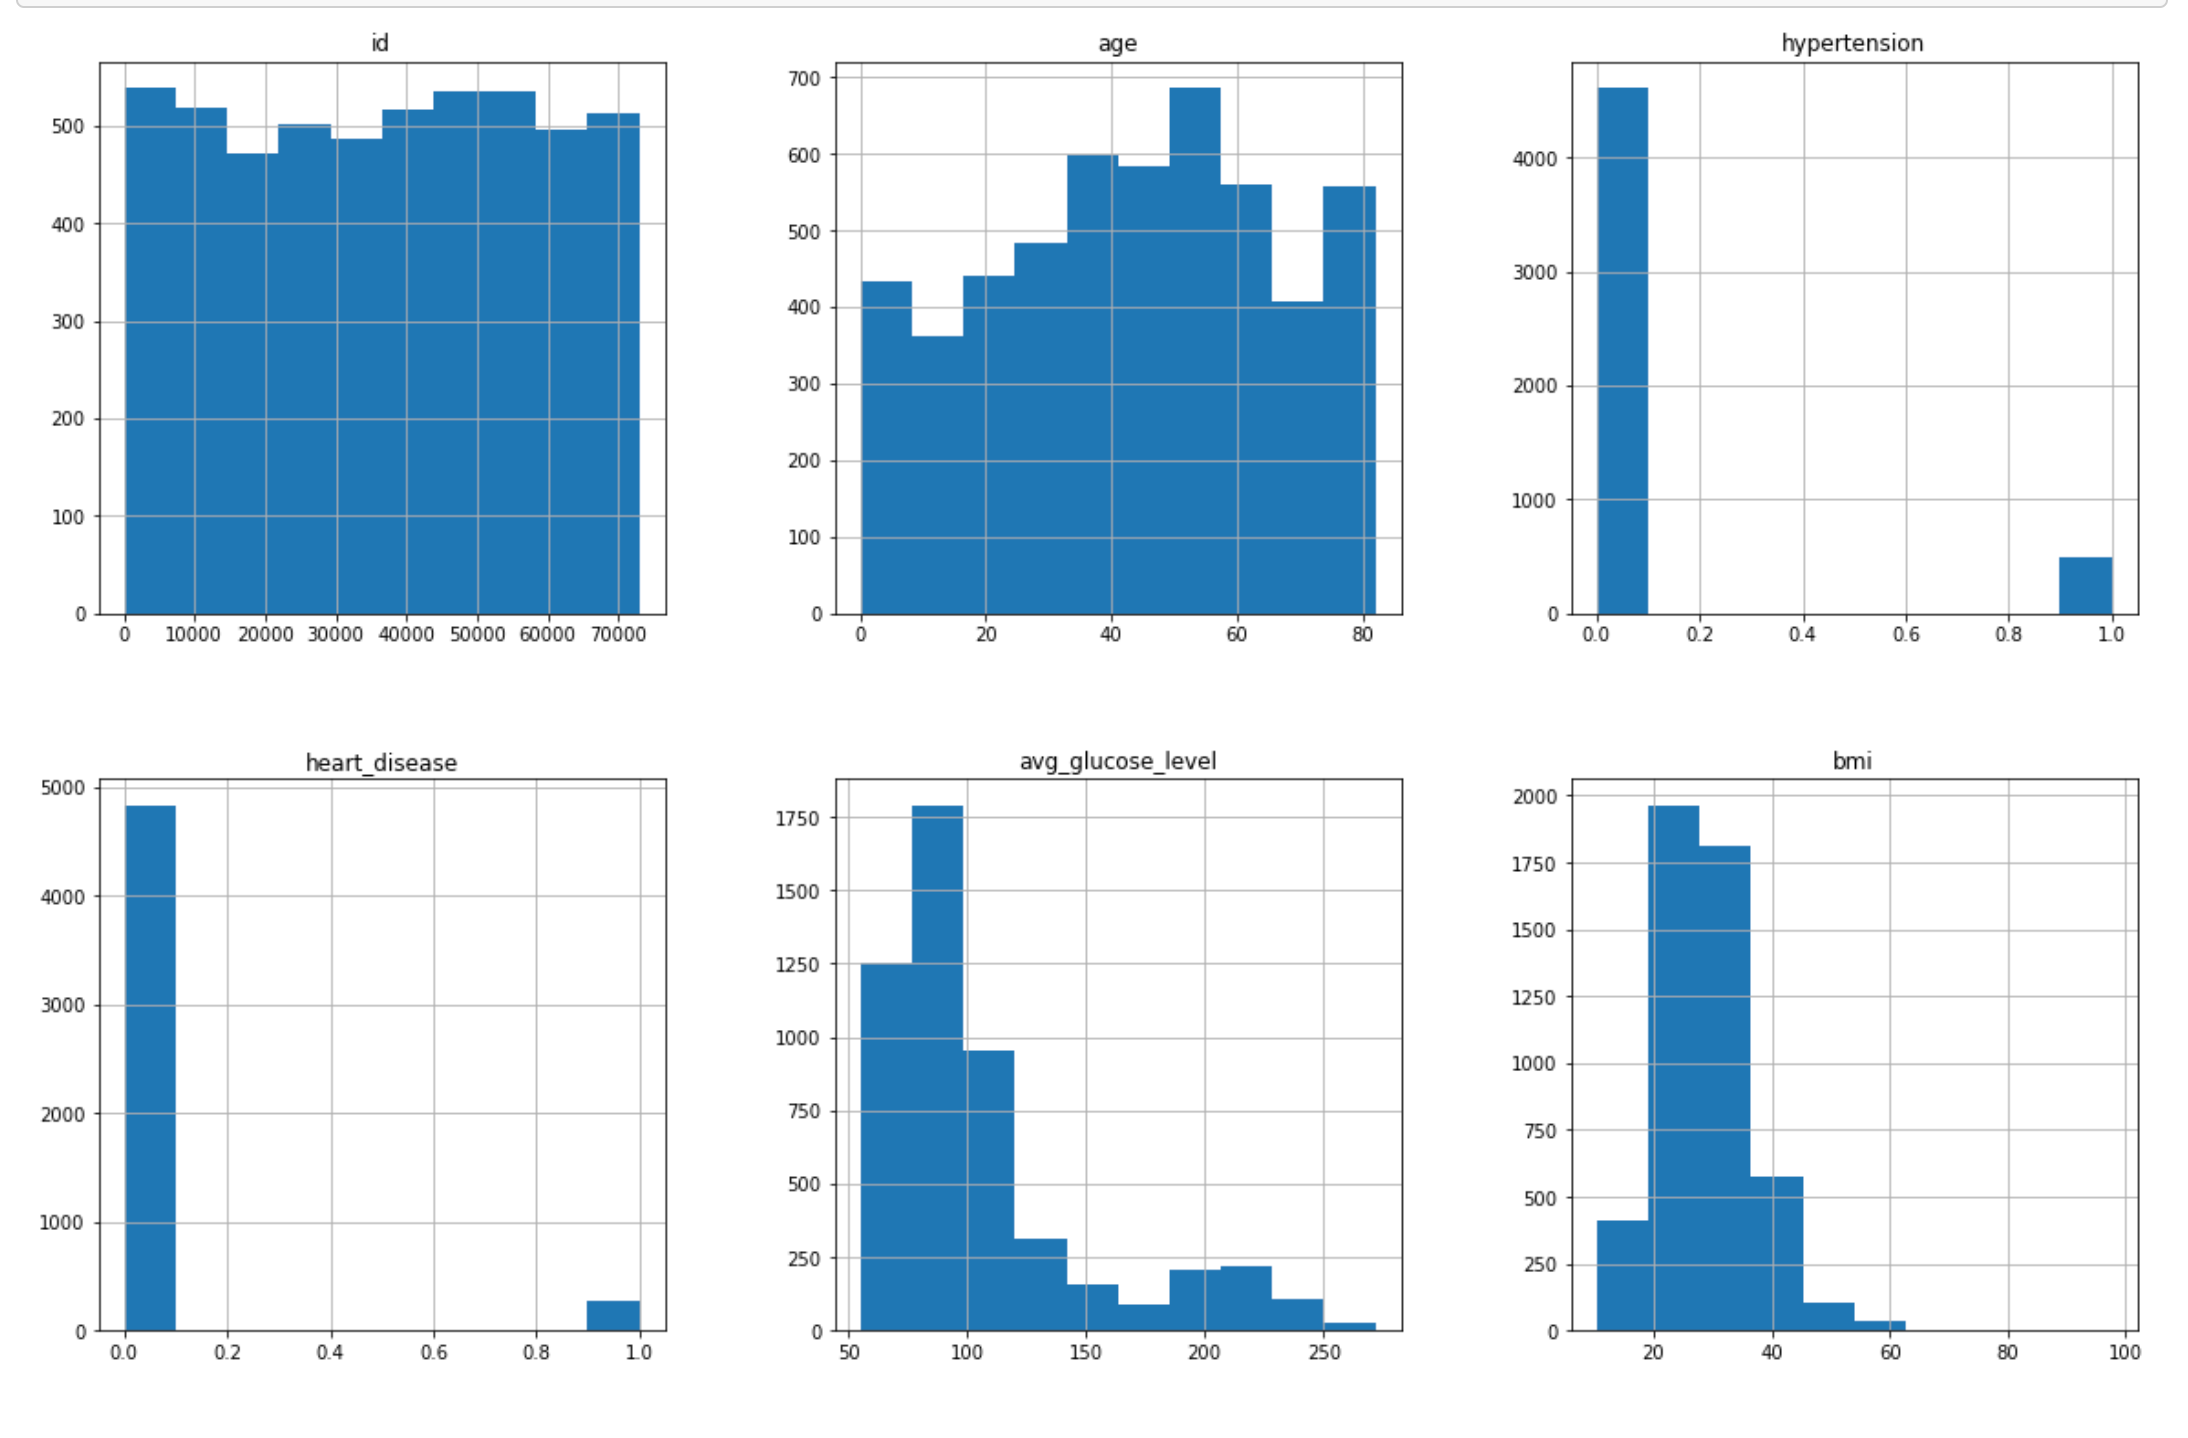
\includegraphics[width=1\linewidth]{Data1}
        \caption{Initial Feature Distribution}
        \label{fig:Figure1}
    \end{subfigure}
    \begin{subfigure}[t]{0.3\textwidth}
        \centering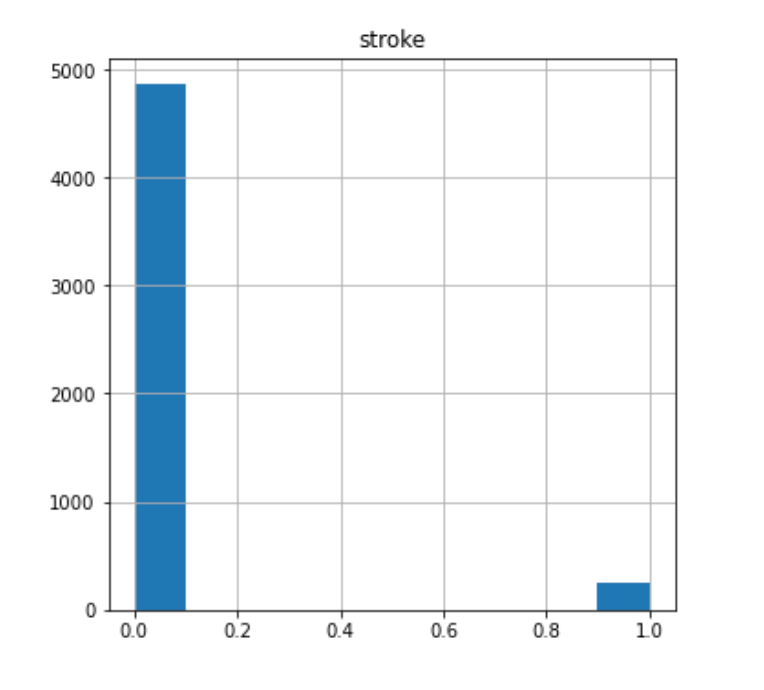
\includegraphics[width=1\linewidth]{Data2}
        \caption{Initial Label Distribution}
        \label{fig:Figure2}
    \end{subfigure}
\end{figure}

\noindent To fix these issues, we performed feature engineering \cite{Stroke_Prediction}. We filled the missing values with that features average result and discarded any unnecessary columns. We then changed the categorical data to numerical data. To fix the imbalance issue, we used the Synthetic Minority Oversampling Technique (SMOTE), which works by selecting examples that are close in the feature spaces, draws a line between the examples in the feature space, and draws a new sample at a point along that line. We also standardized the data by computing the following equation on our features $X$:

\begin{equation}
    \label{eq:Equation1}
    X_{standardized} = \dfrac{X - \mu(X)}{\sigma(X)}
\end{equation}

Where $\mu(X)$ is the mean of $X$, and $\sigma(X)$ is the standard deviation of $X$.\\

\noindent Figures \ref{fig:Figure3} and \ref{fig:Figure4} show feature correlations before and after: replacing N/A values, converting categorical data to discrete data, and standardizing data using Equation \eqref{eq:Equation1}:

\begin{figure}[H]
    \centering
    \begin{subfigure}[t]{.85\textwidth}
        \centering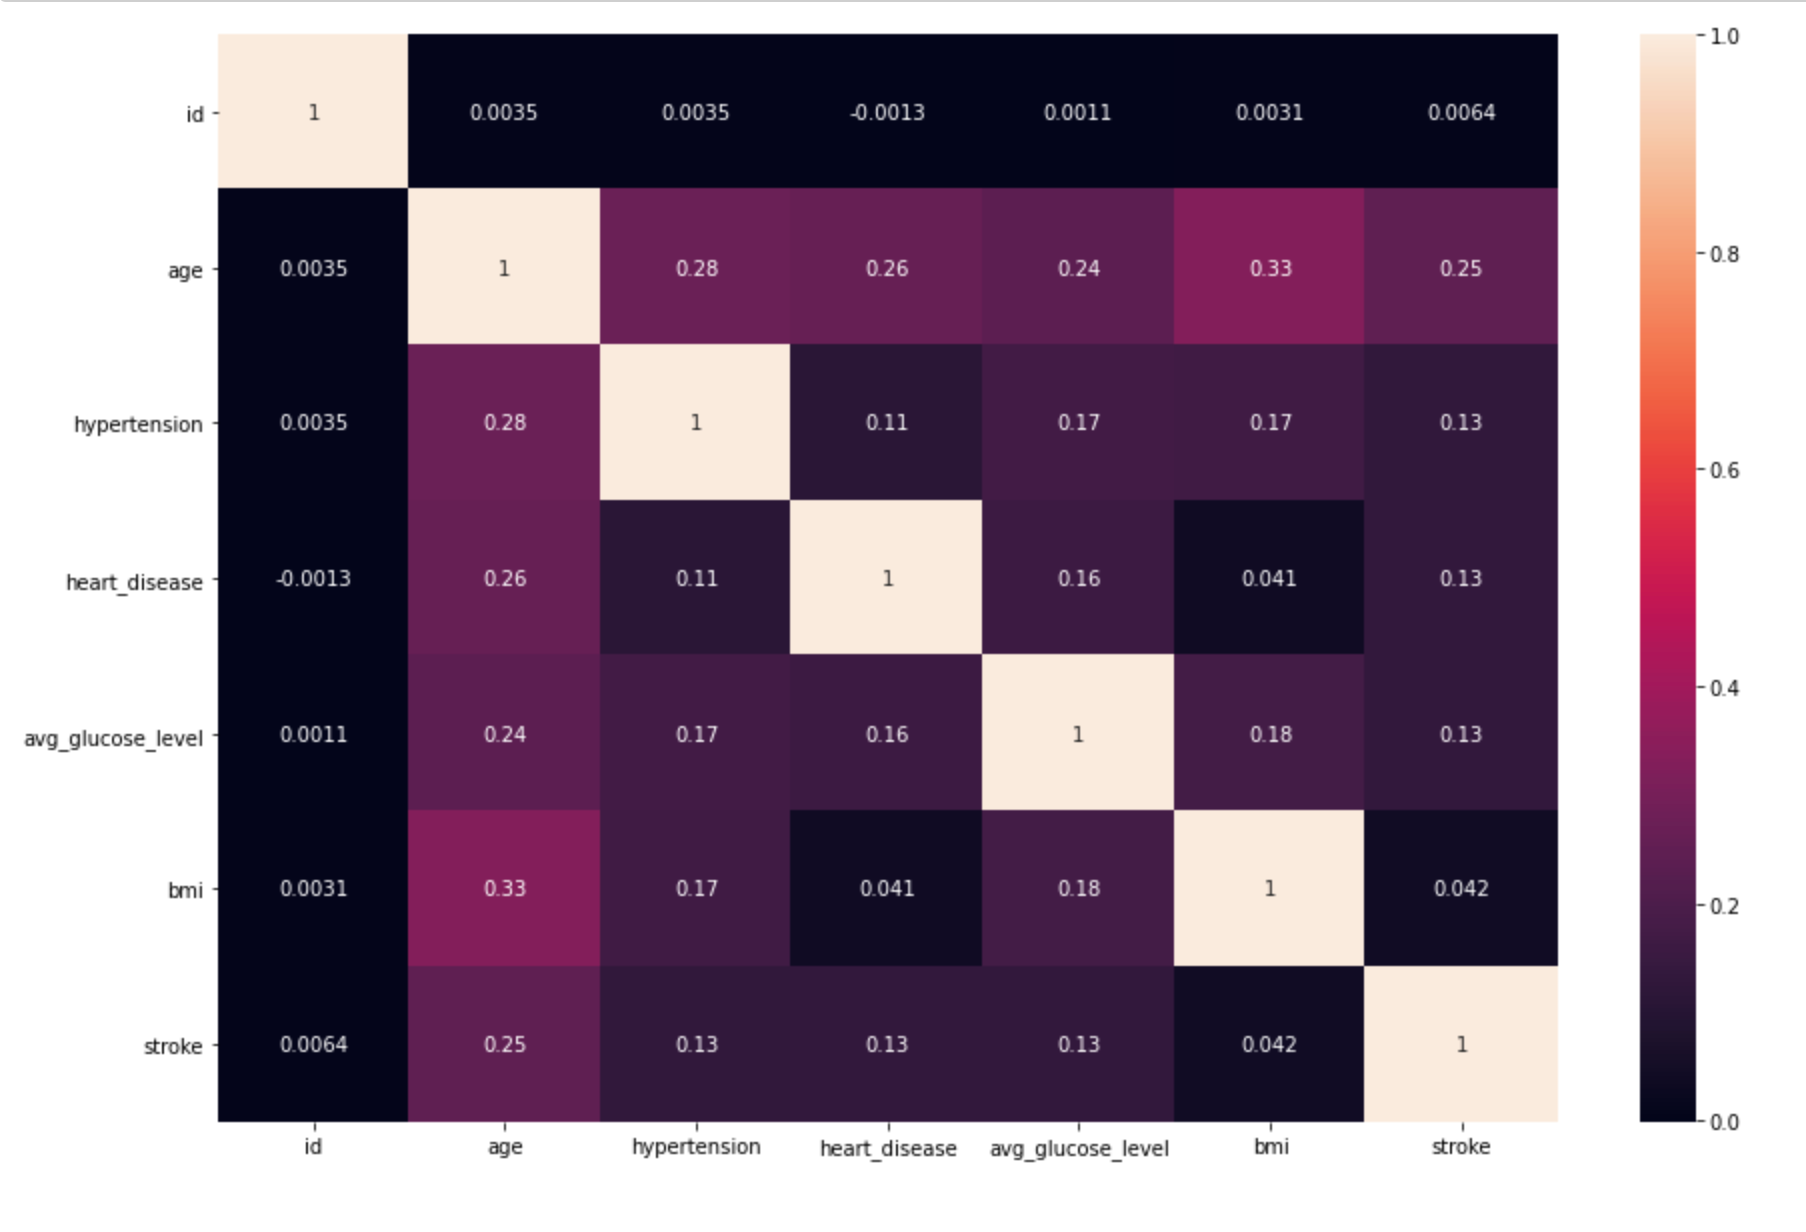
\includegraphics[width=1\linewidth]{Data3}
        \caption{Initial Covariance Matrix}
        \label{fig:Figure3}
    \end{subfigure}\\
    \begin{subfigure}[t]{.85\textwidth}
        \centering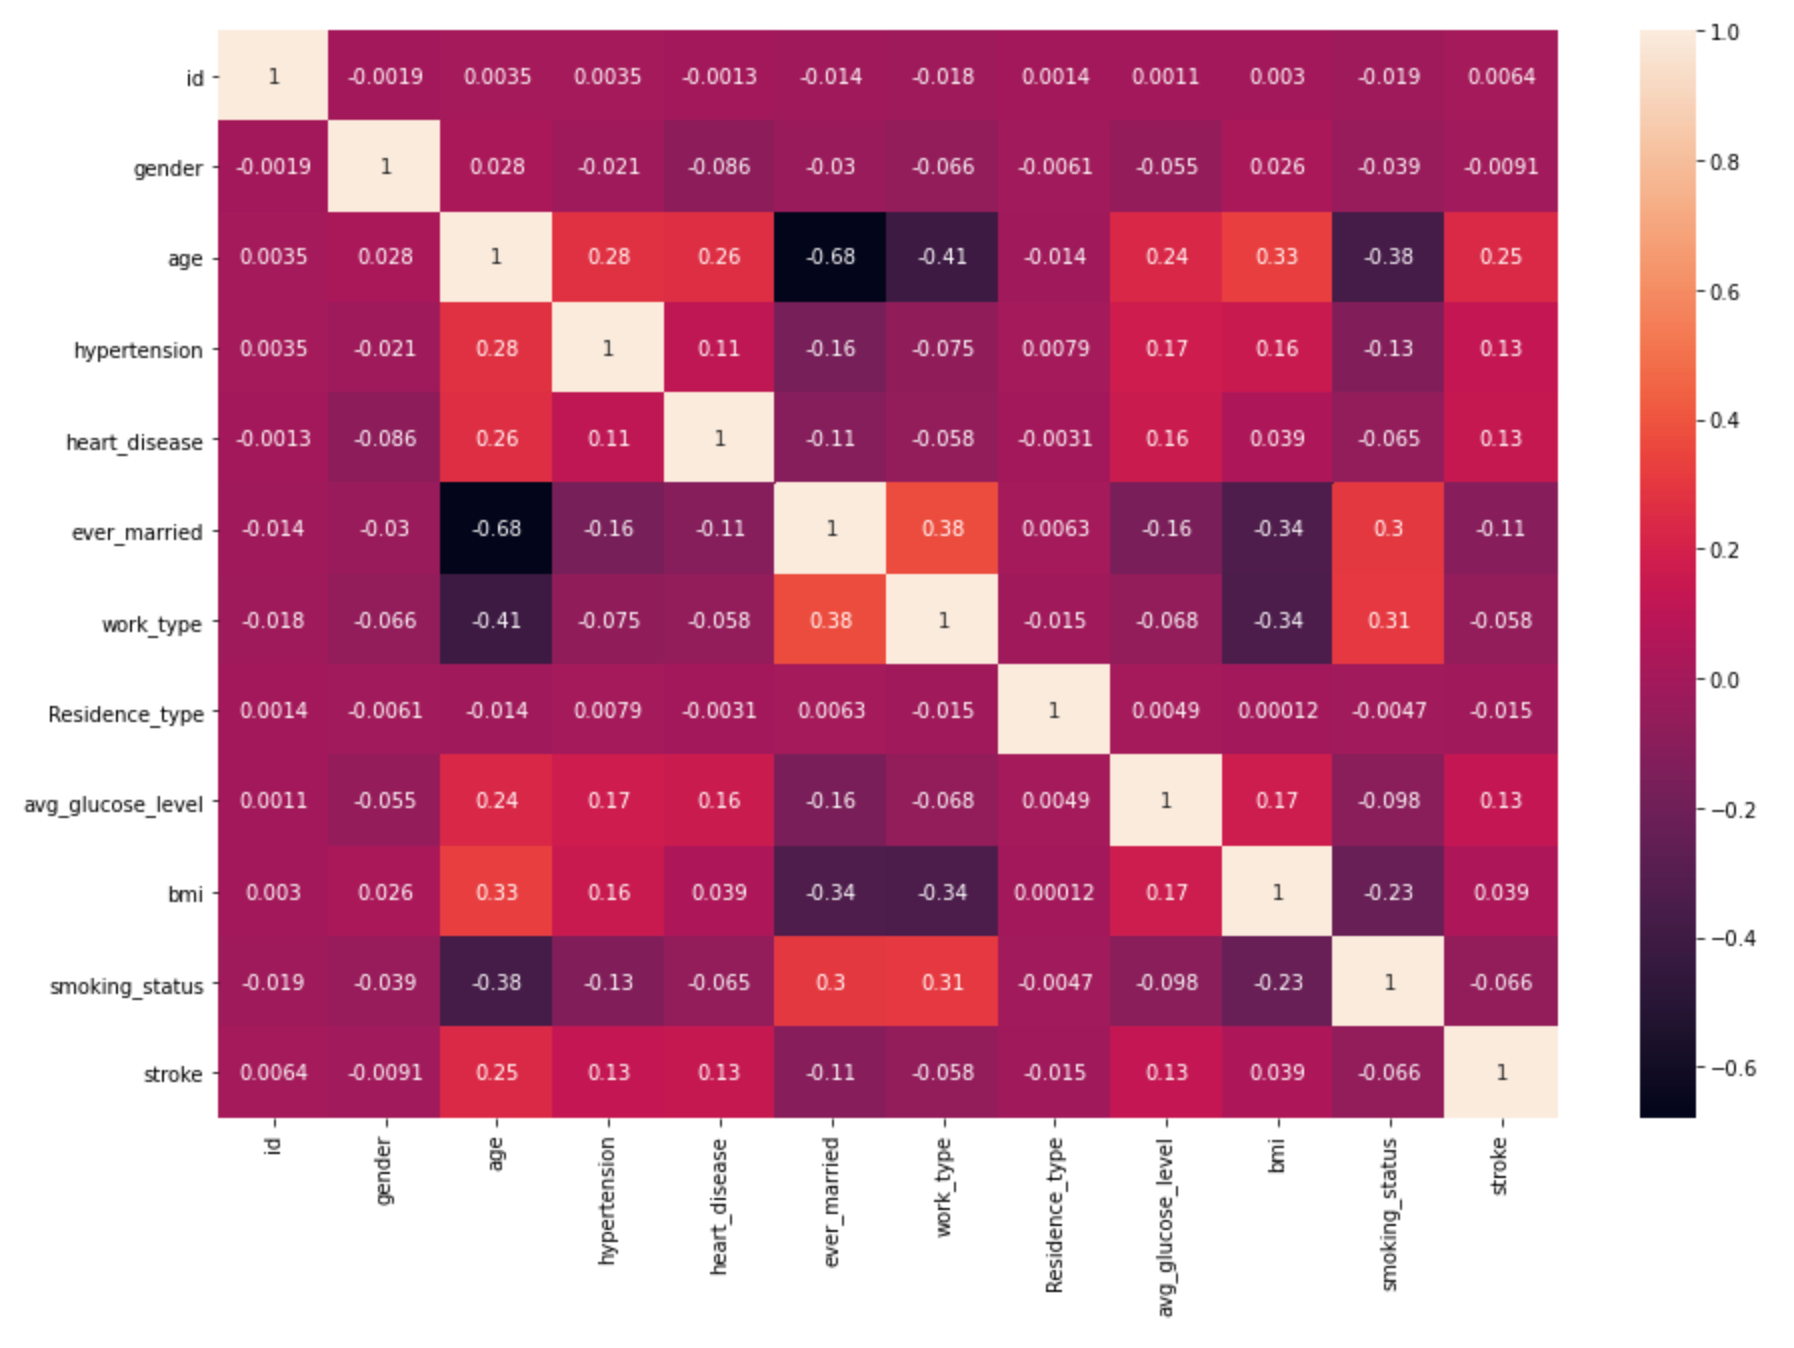
\includegraphics[width=1\linewidth]{Data4}
        \caption{Final Covariance Matrix}
        \label{fig:Figure4}
    \end{subfigure}
\end{figure}

\subsection{Picking Models}
\label{sec:methodology:Picking Models}

With the feature engineering and SMOTE applied to the data, we are ready to proceed. Given the nature of the data, we are facing a supervised learning problem, more specifically a classification problem. Given the severity of the issue at hand, we wanted to compare some more basic classification algorithms, like Logistic Regression \cite{Logistic_Regression}, and see how it would fare against different discriminative algorithms such as SVMs \cite{SVMs} and Decision Trees. In addition, we wanted to find out which features mattered the most in this case, which is the Random Forest algorithm was picked out of all possible Decision Tree based algorithms. 
    \section{Methods}
\label{sec:methods}

\subsection{Logistic Regression}
\label{sec:methods:Logistic Regression}

The Logistic Regression Model is a statistical model that is used to solve classification problems and basically models the probability of a certain class or event happening. In this case, we will be using it to predict whether a person with certain features will get a stroke or not. We will be testing it with both batch gradient descent and stochastic gradient descent. We will also explore k-folding and seeing the effects it might have on the model's results.

\subsubsection{Batch Gradient Descent}
\label{sec:methods:Logistic Regression Model:Batch Gradient Descent}
For this model, I split the data 2/3 for the training set and 1/3 for the testing set. I set random initial values for theta, which are the parameters, and used a learning rate $\eta$ of 0.01. N is the number of observations. This model ran until the absolute value change in the loss of data was less than $2^{-23}$ or after 1,500 iterations had passed.\\

While the model ran, it:
\begin{itemize}
    \item Updated the parameters (theta) using batch gradient descent. Batch gradient descent computes the gradient on the whole dataset. To minimize the cost function and find the optimal solution, we need to run the gradient descent on each parameter $\theta_{j}$:

    \begin{equation}
        \label{eq:Equation2}
        \theta_{j} \leftarrow \theta_{j} - \eta \dfrac{\partial}{\partial{\theta_{j}}} J(\theta)
    \end{equation}

    Where the value of the gradient in Equation \eqref{eq:Equation2} is:

    \begin{equation}
        \label{eq:Equation3}
        \dfrac{\partial}{\partial{\theta_{j}}} J(\theta) = \dfrac{1}{N} \sum_{i = 1}^{N} \Big(h_{\theta}(x^{(i)}) - y^{(i)}\Big)x_{j}^{(i)}
    \end{equation}

    In Equation \eqref{eq:Equation3}, $h_{\theta}(x^{(i)})$ is the sigmoid function, or logistic function. It maps input values to a limited interval. It squeezes any number in $\mathbb{R}$ to the open interval $(0, 1)$, so it is well suited for classification purposes. This hypothesis function approximates the probability of the actual output being equal to 1 and is equivalent to:

    \begin{equation}
        \label{eq:Equation4}
        P(y = 1 \ | \ \theta,x) = \dfrac{1}{1 + e^{-\theta^{T}x}}
    \end{equation}

    Therefore, using Equation \eqref{eq:Equation4}, our sigmoid function is defined as:

    \begin{equation}
        \label{eq:Equation5}
        h_{\theta}(x^{(i)}) = \dfrac{1}{1 + e^{-\theta^{T}x^{(i)}}}
    \end{equation}

    Plugging Equation \eqref{eq:Equation5} into the gradient descent function, we get the final formula for updating the parameters using batch gradient descent:

    \begin{equation}
        \label{eq:Equation6}
        \theta_{j} \leftarrow \theta_{j} - \dfrac{\eta}{N} \sum_{i = 1}^{N} \Big(h_{\theta}(x^{(i)}) - y^{(i)}\Big)x_{j}^{(i)}
    \end{equation}

    Equation \eqref{eq:Equation6} can then be vectorized into easier terms, for code optimizations:

    \begin{equation}
        \label{eq:Equation7}
        \theta \leftarrow \theta - \dfrac{\eta}{N}X^{T}\Big(h_{\theta}(X) - Y\Big)
    \end{equation}

    \item Computed the loss of the data using the logistic regression cost function. The cost function basically summarizes how well the model is behaving - the smaller the value is, the better. Since we’re dealing with a binary classification problem, we define the cost for the two cases separately:

    \begin{equation}
        \label{eq:Equation8}
        J(\theta) =
        \begin{cases}
            -\ln(h_{\theta}(x)) & y = 1\\
            -\ln(1 - h_{\theta}(x)) & y = 0
        \end{cases}
    \end{equation}

    Equation \eqref{eq:Equation8} can be simplified to:

    \begin{equation}
        \label{eq:Equation9}
        J(\theta) = -y^{(i)}\ln(h_{\theta}(x)) - (1 - y^{(i)})\ln(1 - h_{\theta}(x))
    \end{equation}

    For N observations, we modify Equation \eqref{eq:Equation9} to:

    \begin{equation}
        \label{eq:Equation10}
        J(\theta) = -\dfrac{1}{N} \sum_{i = 1}^{N} \Big(y^{(i)}\ln(h_{\theta}(x)) + (1 - y^{(i)})\ln(1 - h_{\theta}(x))\Big)
    \end{equation}

    Equation \eqref{eq:Equation10} can then be vectorized into easier terms, for code optimizations:

    \begin{equation}
        \label{eq:Equation11}
        J(\theta) = -\dfrac{1}{N} \Big(Y^{T} \ln(h_{\theta}(X)) + (1 - Y)^{T}\ln(1 - h_{\theta}(X))\Big)
    \end{equation}
\end{itemize}

\noindent Like stated above, this while-loop ran until either it created ideal parameters (absolute value change in the loss of data was less than $2^{-23}$) or until 1,500 iterations happened.

\subsubsection{Stochastic Gradient Descent}
\label{sec:methods:Logistic Regression Model:Stochastic Gradient Descent}

Then, we switched out the batch gradient descent for stochastic gradient descent. Stochastic gradient descent computes the gradient using a random instance at a single time, so it’s typically much faster than batch gradient descent. Algorithm \eqref{alg:Algorithm1} shows the pseudocode:

\begin{algorithm}
    \caption{Stochastic Gradient Descent}
    \label{alg:Algorithm1}
    \begin{algorithmic}[1]
        \ENSURE $m > 0$
        \FOR{$i$ in range($m$)}
        \STATE{$\theta_{j} \leftarrow \theta_{j} + \eta(\hat{y} - y^{(i)})X_{j}^{(i)}$}
        \ENDFOR
    \end{algorithmic}
\end{algorithm}

\subsubsection{K-Folds Cross Validation}
\label{sec:methods:Logistic Regression Model:K-Folds Cross Validation}

Our last stage with logistic regression was to see how the model worked in k-fold cross validation. Cross validation is a resampling, statistical method used to estimate the skill of a model. $k$ refers to the number of groups that a given data set will be split into. Once the data is split, each group will get a chance to be the testing set and the data will be put through both the logistic regression with batch gradient descent and stochastic gradient descent. Algorithm \eqref{alg:Algorithm2} shows the pseudocode:

\begin{algorithm}
    \caption{K-Folds Cross Validation}
    \label{alg:Algorithm2}
    \begin{algorithmic}[2]
        \ENSURE $k > 1$
        \STATE{Randomly shuffle the dataset}
        \STATE{Split the dataset into k groups}
        \FOR{each unique group}
        \STATE{Take the group as the testing set}
        \STATE{Use the remaining groups as the training set}
        \STATE{Perform logistic regression with the training and testing set}
        \STATE{Compute and save the accuracy, precision, recall and f1 measure in an array}
        \ENDFOR
        \STATE{Display the accuracy, precision, recall and f1 measure arrays for each fold}
    \end{algorithmic}
\end{algorithm}

\subsection{Support Vector Machines}
\label{sec:methods:Support Vector Machines}

The Support Vector Machine (SVM) is a supervised learning model that can be used to solve classification problems. The SVM model finds a hyperplane that distinctly classifies data points in an $N$-dimensional space, where $N$ is the number of features. For our dataset, 10 features are being used to predict whether a person will get a stroke or not. This model chooses the best hyperplane that separates the data into positive and negative values and is the furthest away from the closest data points in order to classify the data points. For the binary class label, the dataset classified 0 as patients who did not have a stroke and 1 as patients who had a stroke. For the SVM model, 0 is mapped to $-1$ and 1 is mapped to $+1$.\\

\noindent The hyperplane is found by minimizing a cost function to find the optimal weights (w) and the intercept (b). The SVM model is defined as:

\begin{equation}
    \label{eq:Equation12}
    f(x) = \mathrm{sgn}(wx + b)
\end{equation}

\noindent A cost function measures how the model is doing in terms of finding a hyperplane that separates the negative and positive data points with the biggest margin possible while keeping the misclassification of the data as low as possible. For the SVM algorithm, we decided to minimize the cost function by using stochastic gradient descent. By expanding upon Equation \eqref{eq:Equation12}, the formula is given below:

\begin{equation}
    \label{eq:Equation13}
    J(w) = \dfrac{1}{2} \lVert w \rVert^2 + \dfrac{C}{N} \sum_{i = 1}^{N} \mathrm{max}(0, 1 - y^{(i)}(wx^{(i)} + b))
\end{equation}

\noindent Where max($0, 1 - y^{(i)}(wx^{(i)} + b)$) is the hinge loss function. A hinge loss function is a loss function that is used for binary classification. The gradient of Equation \eqref{eq:Equation13} is calculated as follows:

\begin{equation}
    \label{eq:Equation14}
    \dfrac{\partial}{\partial{w}}J(w) = \dfrac{1}{N} \sum_{i = 1}^{N}
    \begin{cases}
        w & \mathrm{max}(0, 1 - y^{(i)}(wx^{(i)} + b)) = 0\\
        w - Cy^{(i)}x^{(i)} & \mathrm{max}(0, 1 - y^{(i)}(wx^{(i)} + b)) \neq 0
    \end{cases}
\end{equation}

\noindent For the stochastic gradient descent algorithm, the maximum number of iterations is set to 2048, the learning rate is set to 0.000001 and the cost threshold is set to 0.01. The model will train the data until the model starts to converge, i.e., when there is no significant decrease in the current cost when compared to the previous cost.

\subsection{Random Forest}
\label{sec:methods:Random Forest}

Random forest, as the "forest" part of the name implies, consists of a large number of individual Decision Trees (DTs) that operate as an ensemble. Each individual tree in the random forest spits out a class prediction and the class with the most votes becomes our model’s prediction. For some background, we picked this route because DTs, while still discriminative in nature, perform classification in a manner that is fundamentally different than other algorithms like Logistic Regression and SVMs. Each internal node tests an attribute, each branch is an attribute value, and each leaf assigns a classification. While the latter two algorithms use metric cost functions between features (Euclidean/Manhattan Distance) and sometimes a kernel function (Gaussian/Logistic Kernel), Decision Trees apply a sequence of decisions or rules that often depend on a single variable at a time.\\

\noindent As we run through using a Decision Tree, we start at the root node, check on a feature and value, and make a decision from there, taking us to the next level of the tree. The way we decide which features we split on is through information gain, which is based on sample entropy. Sample Entropy (Equation \eqref{eq:Equation15}) and Information Gain (Equation \eqref{eq:Equation16}) can be computed as follows:

\begin{equation}
    \label{eq:Equation15}
    H(Y) = - \sum_{i=1}^N P(Y=y_i) \log_2 P(Y=y_i)
\end{equation}

\begin{equation}
    \label{eq:Equation16}
    I(Y) = H(Y) - \sum_{i = 1}^{N} \dfrac{P(Y = y_{i})}{P(Y)} H(Y_{i})
\end{equation}

\noindent The easiest way to run through our own tree would be to do this is if we deal with binarized data and construct binary DTs, for example:

\begin{forest}
    for tree={l sep=30pt, parent anchor=south, align=center}
    [$x_1$,
    [$x_2$, label=T,
    [$+$, label=T],
    [$+$, label=F]
    ],
    [$x_2$, label=F,
    [$+$, label=T],
    [$-$, label=F]
    ]
    ]
\end{forest}

\noindent However, since determining the optimal value of continuous data to split on is no easy feat, all unique values were used instead. While every tree with a branching factor greater than two can be recomposed into an equivalent binary tree, so we decided to do this to reduce recursive complexity. Now that we have a way to decide which feature to split on, we want to first pick the features that yield the highest Information Gain, or the lowest sample entropy. This is because the entropy is a measure of the "randomness" of a system, so we want to find the most deterministic features. Algorithm \eqref{alg:Algorithm3} shows us how to find a proper decision tree using the ID3 (Iterative Dichotomiser 3):

\begin{algorithm}[H]
    \caption{ID3}
    \label{alg:Algorithm3}
    \begin{algorithmic}[3]
        \IF{No Data Left}
        \RETURN{mode(Y)}
        \ENDIF
        \IF{All Y values are equal}
        \RETURN{Y[0]}
        \ENDIF
        \IF{Only 1 feature in features}
        \RETURN{mode(Y[feature])}
        \ENDIF
        \STATE{Find Best Feature and Delete from Features}
        \STATE{Find Data above and below Value associated with Feature}
        \RETURN{[ID3(below, Features), ID3(above, Features)]}
    \end{algorithmic}
\end{algorithm}

\noindent From there, we have constructed our DT using the ID3 algorithm. From here, we need to cover the idea behind a Random Forest. Random Forests do what is called \textbf{Bagging}, otherwise known as Bootstrap Aggregation. In essence, this means that in a collection of trees, each tree structure is different when subjected to random sampling. This is a policy that takes advantage of how sensitive a decision tree is to the data it is trained on (due to DT's natural tendency of high variance) \cite{Random_Forest}. Algorithm \eqref{alg:Algorithm4} shows us how to construct a Random Forest:

\begin{algorithm}
    \caption{Random Forest}
    \label{alg:Algorithm4}
    \begin{algorithmic}[4]
        \FOR{i in range(num\_trees)}
        \STATE{randomly sample from data}
        \STATE{randomly sample from features}
        \STATE{append ID3(data, features) to forest}
        \ENDFOR
        \RETURN{forest}
    \end{algorithmic}
\end{algorithm}

To classify the data, we then recurse through the tree using the data we wish to look at, and return the classification yielded by the leaf node we land on.
    \section{Evaluation}
\label{sec:evaluation}

For reference, Accuracy is defined as:

\begin{equation}
    \label{eq:Equation17}
    \dfrac{TP + TN}{TP + FP + TN + FN}
\end{equation}

Precision is defined as:

\begin{equation}
    \label{eq:Equation18}
    \dfrac{TP}{TP + FP}
\end{equation}

Recall is defined as:

\begin{equation}
    \label{eq:Equation19}
    \dfrac{TP}{TP + FN}
\end{equation}

F1-Score is defined as:

\begin{equation}
    \label{eq:Equation20}
    \dfrac{2\eqref{eq:Equation18}\eqref{eq:Equation19}}{\eqref{eq:Equation18} + \eqref{eq:Equation19}} = \dfrac{TP}{TP + \frac{1}{2}(FP + FN)}
\end{equation}

Where:
\begin{itemize}
    \item $TP$ is the count of where both predictions and true values are positive
    \item $FP$ is the count of where predictions are positive but true values are negative
    \item $TN$ is the count of where both predictions and true values are negative
    \item $FN$ is the count of where predictions are negative but true values are positive
\end{itemize}

\subsection{Logistic Regression}
\label{sec:evaluation:Logistic Regression}
After running the logistic regression file multiple times, we noticed that the results for each situation between each run were very similar. So, we decided to include the results from one run to maintain space. On the left-hand side of Table \ref{tab:Table1}, you can see the different experiment setting each logistic regression model created. Table \ref{tab:Table1} shows the accuracy, precision, recall and F1-measure results. The accuracy for the Logistic Regression Built in function was around 81.74\%. All the models worked well in terms of accuracy, but the one that came the closest was the ones that involved k-fold cross validation. These tests almost always had an 80\% or higher accuracy rate. The same could be said for precision and F1-measure. However, for recall, the models without k-fold cross validation had a more similar result to the built in function, which was around 85\%.\\

\noindent Between Batch gradient descent and stochastic gradient descent, there wasn’t that much of a difference in the results. They were either the same percentage, or off by 1 point. K-Fold Cross Validation seems to have a huge effect in making the model more precise. It is very clear in these results that it’s better to do k-fold cross validation than not in order to get more accurate results. This makes sense, since it creates multiple training groups and can create a better model as a result of this.\\

\noindent Table \ref{tab:Table2} shows the True Positive, False Positive, True Negative and False Negative Results for the Logistic Regression Model in the different experimental settings.

\begin{table}[ht]
    \centering
    \begin{tabular}{|l|l|l|l|l|}
        \hline
        \textbf{Algorithm}                   & \textbf{Accuracy} & \textbf{Precision} & \textbf{Recall} & \textbf{F1-Score} \\
        \hline
        \textbf{Batch Gradient Descent}      & 77.625            & 73.546             & 86.827          & 79.637            \\
        \textbf{Stochastic Gradient Descent} & 77.999            & 74.397             & 85.899          & 79.736            \\
        \textbf{K-Folds = 5 (BGD)}           & 80.905            & 77.929             & 86.259          & 81.876            \\
        \textbf{K-Folds = 5 (SGD)}           & 80.864            & 77.655             & 86.662          & 81.910            \\
        \textbf{K-Folds = 10 (BGD)}          & 80.936            & 77.718             & 86.779          & 81.972            \\
        \textbf{K-Folds = 10 (SGD)}          & 81.440            & 77.968             & 87.695          & 82.523            \\
        \textbf{Sci-Kit Learn}               & 81.739            & 79.988             & 85.034          & 82.434            \\
        \hline
    \end{tabular}
    \caption{Metrics of Different Algorithms (Averaged)}
    \label{tab:Table1}
\end{table}

\begin{table}[ht]
    \centering
    \begin{tabular}{|l|l|l|l|l|}
        \hline
        \textbf{Algorithm}                   & \textbf{TP} & \textbf{FP} & \textbf{TN} & \textbf{FN} \\
        \hline
        \textbf{Batch Gradient Descent}      & 1404        & 505         & 1087        & 213         \\
        \textbf{Stochastic Gradient Descent} & 1389        & 478         & 1114        & 228         \\
        \textbf{K-Folds = 5 (BGD)}           & 838.6       & 237.6       & 734.2       & 133.6       \\
        \textbf{K-Folds = 5 (SGD)}           & 842.6       & 242.4       & 729.4       & 129.6       \\
        \textbf{K-Folds = 10 (BGD)}          & 421.6       & 121         & 365.1       & 64.3        \\
        \textbf{K-Folds = 10 (SGD)}          & 426.1       & 120.5       & 365.5       & 59.9        \\
        \hline
    \end{tabular}
    \caption{Confusion Matrix Results (Averaged)}
    \label{tab:Table2}
\end{table}

\subsection{SVMs}
\label{sec:evaluation:SVMs}

Similar to the logistic regression script, for multiple runs of the support vector machine (SVM) script, SVM produced statistics that were very similar for multiple runs. Therefore, results from one run are included in Table \ref{tab:Table3}. This table shows the accuracy, precision, recall, and f1-measure for the SVM algorithm and the built in SVM function. Table \ref{tab:Table4} shows the True Positive, False Positive, True Negative and False Negative Results for the SVM model.

\begin{table}[ht]
    \centering
    \begin{tabular}{|l|l|l|l|l|}
        \hline
        \textbf{Algorithm}     & \textbf{Accuracy} & \textbf{Precision} & \textbf{Recall} & \textbf{F1-Score} \\
        \hline
        \textbf{SVM}           & 78.218            & 74.931             & 84.625          & 79.483            \\
        \textbf{Sci-Kit Learn} & 82.674            & 78.308             & 90.25           & 83.856            \\
        \hline
    \end{tabular}
    \caption{Metrics}
    \label{tab:Table3}
\end{table}

\begin{table}[H]
    \centering
    \begin{tabular}{|l|l|l|l|l|}
        \hline
        \textbf{Algorithm}     & \textbf{TP} & \textbf{FP} & \textbf{TN} & \textbf{FN} \\
        \hline
        \textbf{SVM}           & 1354        & 453         & 1156        & 246         \\
        \textbf{Sci-Kit Learn} & 1444        & 400         & 1209        & 156         \\
        \hline
    \end{tabular}
    \caption{Confusion Matrix Results}
    \label{tab:Table4}
\end{table}

\subsubsection{Precision-Recall Curves}
\label{sec:evaluation:SVMs:Precision-Recall Curves}

Figures \ref{fig:Figure5} and \ref{fig:Figure6} plot the precision (y-axis) against the recall (x-axis).

\begin{figure}[ht]
    \centering
    \begin{subfigure}[t]{.45\textwidth}
        \centering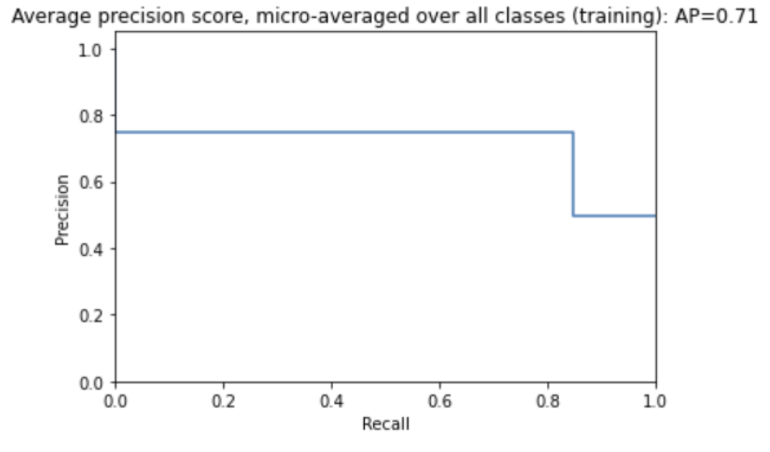
\includegraphics[width=1\linewidth]{PR1}
        \caption{PR Curve of Our Model}
        \label{fig:Figure5}
    \end{subfigure}
    \begin{subfigure}[t]{.45\textwidth}
        \centering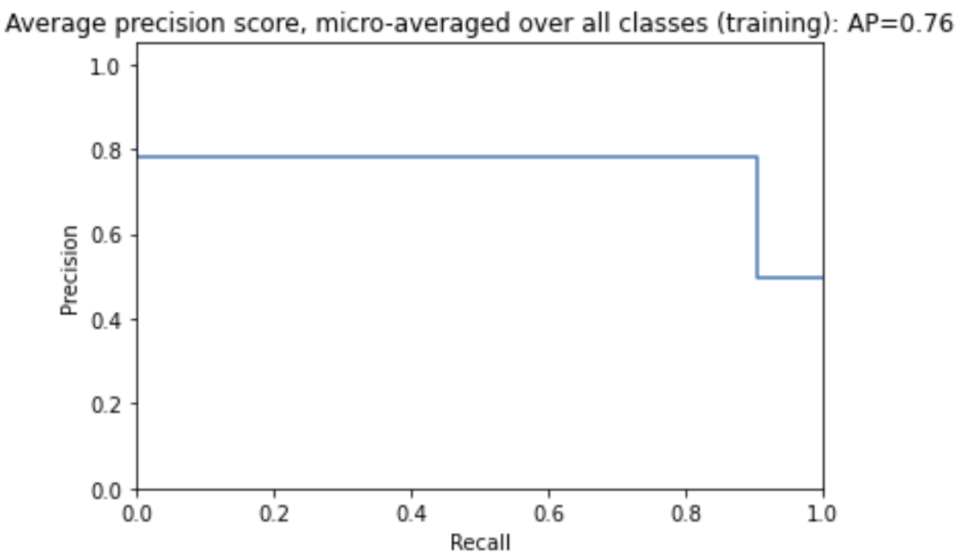
\includegraphics[width=1\linewidth]{PR2}
        \caption{PR Curve of Sci-Kit Learn's Model}
        \label{fig:Figure6}
    \end{subfigure}
\end{figure}

\subsection{Random Forest}
\label{sec:evaluation:Random Forest}

Unlike Logistic Regression and SVMs, our Random Forest model was somewhat flawed as we assumed all data was continuous rather than looking at a mix of continuous and discrete data. Due to this, not was our DT model unnecessarily expensive in both time and space complexities, but it caused our Random Forest model to be not much of an improvement over a regular DT. Table \ref{tab:Table5} and Table \ref{tab:Table6} show the results of ID3 and Random Forest:

\begin{table}[ht]
    \centering
    \begin{tabular}{|l|l|l|l|l|}
        \hline
        \textbf{Algorithm}     & \textbf{Accuracy} & \textbf{Precision} & \textbf{Recall} & \textbf{F1-Score} \\
        \hline
        \textbf{ID3}           & 70.365            & 65.722             & 86.085          & 74.538            \\
        \textbf{Sci-Kit Learn} & 89.685            & 88.503             & 91.404          & 89.93             \\
        \hline
    \end{tabular}
    \caption{ID3 Metrics}
    \label{tab:Table5}
\end{table}

\begin{table}[ht]
    \centering
    \begin{tabular}{|l|l|l|l|l|}
        \hline
        \textbf{Algorithm}     & \textbf{Accuracy} & \textbf{Precision} & \textbf{Recall} & \textbf{F1-Score} \\
        \hline
        \textbf{Random Forest} & 71.206            & 66.651             & 85.776          & 75.014            \\
        \textbf{Sci-Kit Learn} & 94.734            & 93.773             & 95.918          & 94.833            \\
        \hline
    \end{tabular}
    \caption{Random Forest Metrics}
    \label{tab:Table6}
\end{table}
    \section{Conclusion}
\label{sec:conclusion}

\subsection{Overall Analysis}
\label{sec:conclusion: Overall Analysis}
From our data analysis and the graphs we plotted, people over the age of 50 are more likely to get a stroke compared to people under the age of 50. Individuals with hypertension (high blood pressure) are more likely to get a stroke. Males are more prone to a stroke compared to females.\\

\noindent The Logistic Regression model seemed to perform similarly, whether it was created with Batch Gradient Descent or Stochastic Gradient Descent. However, the results very clearly show that running the model with k-folds will significantly increase the accuracy, by at least 3\%. Additionally, the higher the number of folds, the greater the accuracy. For our results, it seemed like Logistic Regression with Stochastic Gradient Descent and with K-Folds = 10 had the most similar results to the built in Scikit Logistic Regression. There is a time drawback for doing higher k-folds, so if getting more accurate results by 3\% is important, then it would take longer to run than Logistic Regression without k-folds.\\

\noindent The built-in SVC function from the Scikit Learn library had higher percentages for accuracy, precision, recall, and f-measure compared to the support vector machine algorithm. The accuracy, precision, and F-measure was better by approximately 4\% for the built-in SVC function compared to the SVM algorithm and the recall was approximately 6\% higher.\\

\noindent Lastly, Random Forest wasn't quite the success story we were hoping to have. With Sci-Kit Learn having over 20\% in nearly every metric, it is clear we need work. Some of the improvements include the binarization of continuous data for complexity purposes, as well as the differentiation of continuous data from discrete data in the ID3 algorithm for better metrics. While Random Forest didn't yield the results we wanted, it was useful in helping us with determining the level of contribution of each feature. Figure \ref{fig:Figure7} shows us the importance of the different features:

\begin{figure}[ht]
    \centering
    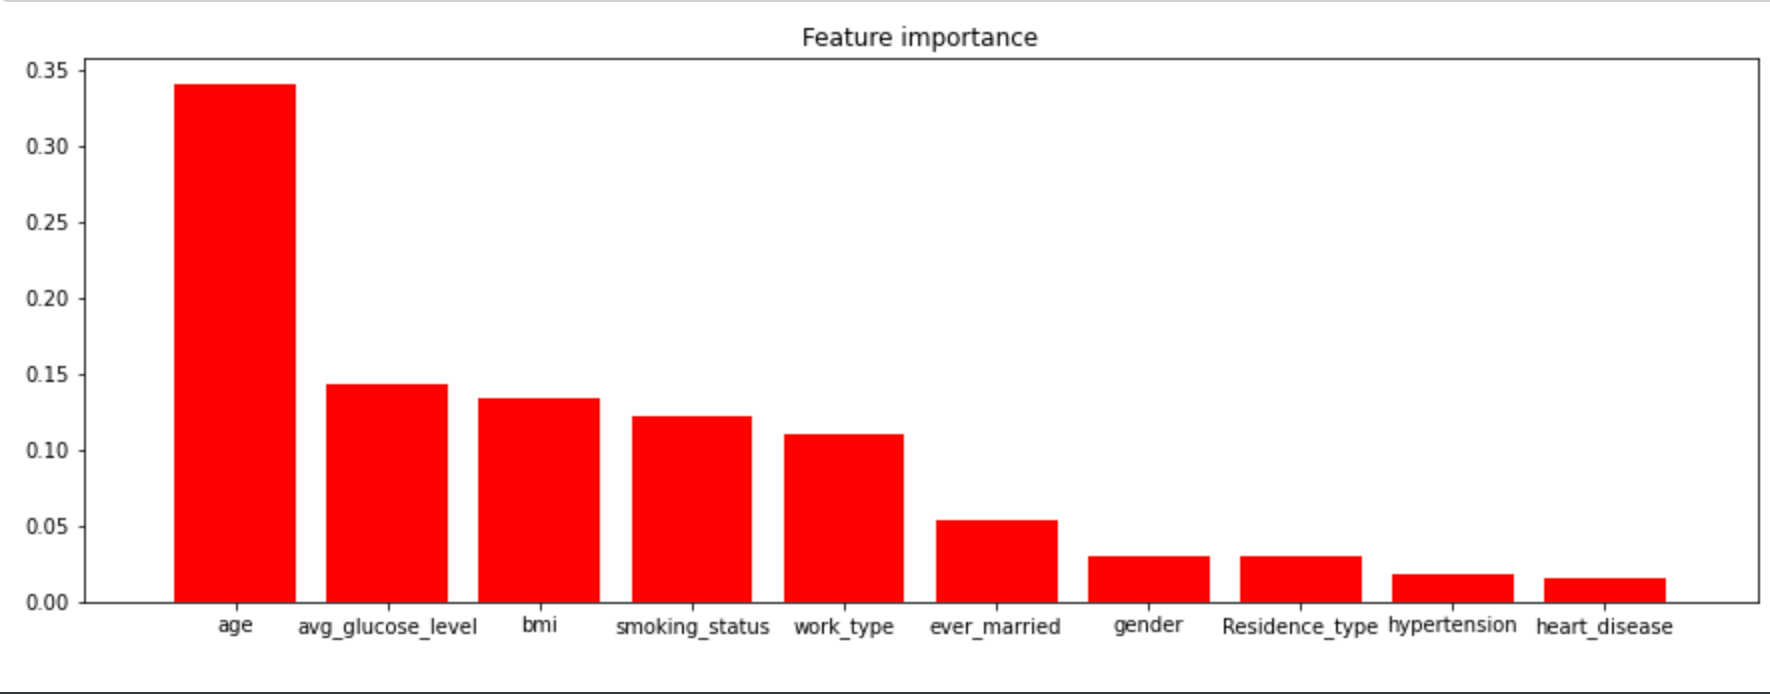
\includegraphics[width=1\linewidth]{Feature_Importances}
    \caption{Feature Importance}
    \label{fig:Figure7}
\end{figure}

\subsection{Future Work}
\label{sec:conclusion: Future Work}


\noindent For future work, we would like to explore the importance of various features to help filter features that are irrelevant or redundant. This would help improve the models which are used to predict whether a patient is likely to have a stroke. In addition, we would like to experiment with finding the optimal learning rate for the stochastic gradient algorithm. Small learning rates tend to converge too slowly, which makes our model too inefficient, whereas large learning rates causes our model to overshoot the minima and diverge. Finding the optimal learning rate will help in lowering the number of iterations in order to find a model with high accuracy.\\

\noindent Some extra conclusions we determined were that, apart from a lot of categories that do not make sense for this context, some of the metrics are flawed. BMI in general is not a good metric to use, so it would be better to measure weight \cite{BMI}. Also, we are unsure if smoking is related to tobacco, cannabis, crack cocaine, or any other drug that can be inflammed and inhaled. Nonetheless, we see that age is clearly the biggest contributor to one's likelihood to suffer a stroke by far.
%\input{sections/appendix}
    \clearpage

%----------------------------------------------------------------------------------------
%	Appendix
%----------------------------------------------------------------------------------------
%\input{sections/appendix}

%----------------------------------------------------------------------------------------
%	Bibliography
%----------------------------------------------------------------------------------------
    \clearpage
    \bibliography{bibliography/references}{}
    \bibliographystyle{plainurl}

\end{document}